\documentclass[a4paperpaper,]{article}
\usepackage{lmodern}
\usepackage{amssymb,amsmath}
\usepackage{ifxetex,ifluatex}
\usepackage{fixltx2e} % provides \textsubscript
\ifnum 0\ifxetex 1\fi\ifluatex 1\fi=0 % if pdftex
  \usepackage[T1]{fontenc}
  \usepackage[utf8]{inputenc}
\else % if luatex or xelatex
  \ifxetex
    \usepackage{mathspec}
  \else
    \usepackage{fontspec}
  \fi
  \defaultfontfeatures{Ligatures=TeX,Scale=MatchLowercase}
\fi
% use upquote if available, for straight quotes in verbatim environments
\IfFileExists{upquote.sty}{\usepackage{upquote}}{}
% use microtype if available
\IfFileExists{microtype.sty}{%
\usepackage[]{microtype}
\UseMicrotypeSet[protrusion]{basicmath} % disable protrusion for tt fonts
}{}
\PassOptionsToPackage{hyphens}{url} % url is loaded by hyperref
\usepackage[unicode=true]{hyperref}
\hypersetup{
            pdfborder={0 0 0},
            breaklinks=true}
\urlstyle{same}  % don't use monospace font for urls
\usepackage{graphicx,grffile}
\makeatletter
\def\maxwidth{\ifdim\Gin@nat@width>\linewidth\linewidth\else\Gin@nat@width\fi}
\def\maxheight{\ifdim\Gin@nat@height>\textheight\textheight\else\Gin@nat@height\fi}
\makeatother
% Scale images if necessary, so that they will not overflow the page
% margins by default, and it is still possible to overwrite the defaults
% using explicit options in \includegraphics[width, height, ...]{}
\setkeys{Gin}{width=\maxwidth,height=\maxheight,keepaspectratio}
\IfFileExists{parskip.sty}{%
\usepackage{parskip}
}{% else
\setlength{\parindent}{0pt}
\setlength{\parskip}{6pt plus 2pt minus 1pt}
}
\setlength{\emergencystretch}{3em}  % prevent overfull lines
\providecommand{\tightlist}{%
  \setlength{\itemsep}{0pt}\setlength{\parskip}{0pt}}
\setcounter{secnumdepth}{0}
% Redefines (sub)paragraphs to behave more like sections
\ifx\paragraph\undefined\else
\let\oldparagraph\paragraph
\renewcommand{\paragraph}[1]{\oldparagraph{#1}\mbox{}}
\fi
\ifx\subparagraph\undefined\else
\let\oldsubparagraph\subparagraph
\renewcommand{\subparagraph}[1]{\oldsubparagraph{#1}\mbox{}}
\fi

% set default figure placement to htbp
\makeatletter
\def\fps@figure{htbp}
\makeatother


\date{}

\begin{document}

\section{Wind-forcing comparison in
INALT20}\label{wind-forcing-comparison-in-inalt20}

Authors: Kristin Burmeister, Franziska Schwarzkopf, Arne Biastoch, Peter
Brandt, Joke Luebbecke, Mark Inall

\section{Aim:}\label{aim}

In this study the difference between the COREv2 (Griffies et al. (2009))
and JRA55-do (Tsujino et al. (2018)) forcing in INALT20 (Schwarzkopf et
al. (2019)) is investigated with respect to the upper wind-driven ocean
circulation in the tropical Atlantic. Where possible, the model outputs
are validated and the analysis is extended by observational data.

\section{Motivation:}\label{motivation}

The COREv2 wind forcing is known to exhibit spurious multidecadal wind
variability (Hurrell and Trenberth, 1998; Fiorino, 2000;, He et al.,
2016). This presumable impacts the multidecadal variability of the
wind-driven circulation in the tropical Atlantic in model simulation
forced by COREv2. The upper wind-driven circulation in the tropical
Atlantic plays a key role in the basin wide distribution of water mass
properties and affects the transport of heat, salt and biogeochemical
components like oxygen (Fig. \ref{fig_schema} and e.g. Schott, McCreary
Jr., and Johnson (2004), Hazeleger and Drijfhout (2006), Oschlies et al.
(2018)). It is an important feature of the Atlantic climate system and
the marine ecology in a warming world. Hence, it is crucial to improve
the understanding of its long-term variability which is largly depending
on model simulation due to sparse observational data coverage in earlier
periods.

\begin{figure}
\centering
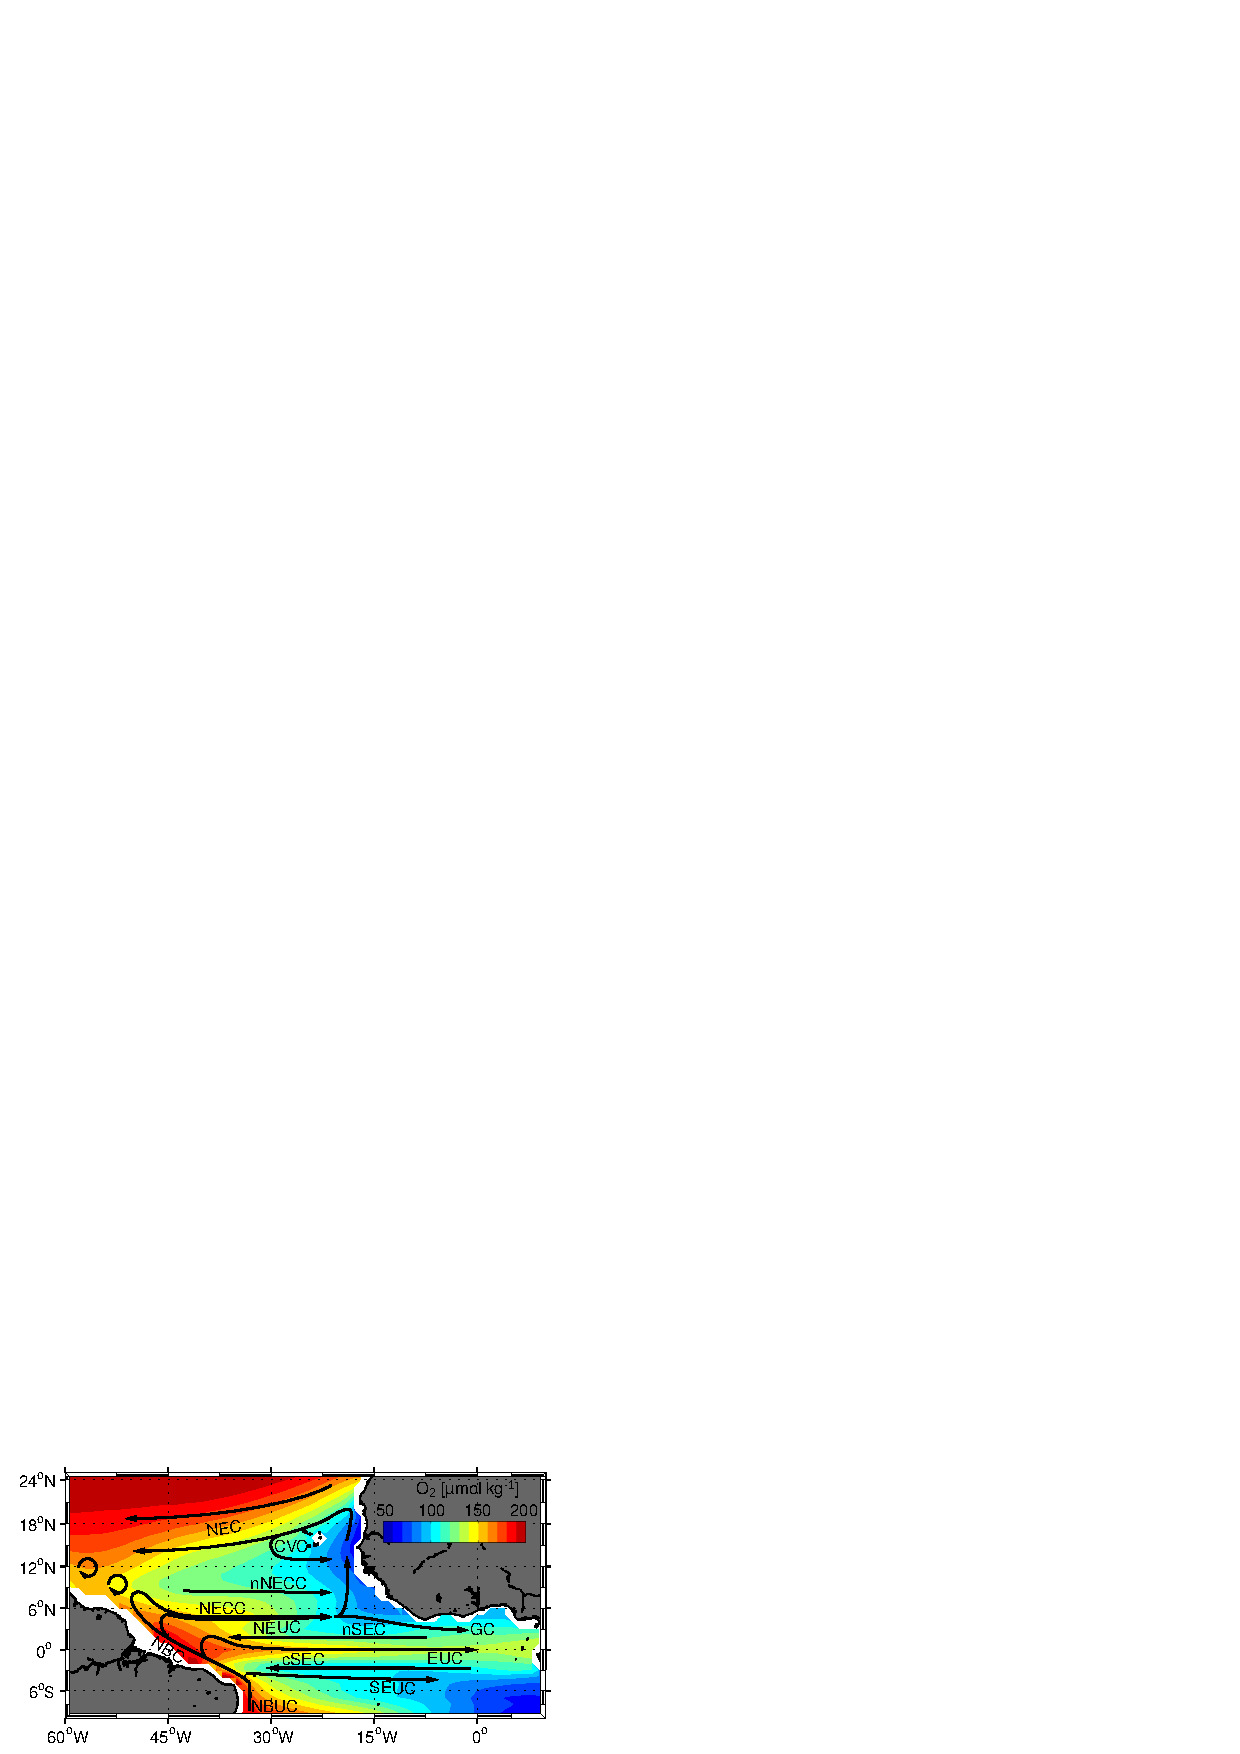
\includegraphics{./figures/from_thesis/f02_schema_MIMOC_100m200m.png}
\caption{Oxygen concentration in \(\mu\)mol\(\,\)kg\(^{-1}\) (shaded
colors) averaged between 100\(\,\)m and 200m depth obtained from MIMOC
(Schmidtko, Stramma, and Visbeck (2017)). Superimposed are surface and
thermocline (about upper 300\(\,\)m) currents (black solid arrows;
adapted from Hahn et al. (2017)): the North Equatorial Current (NEC),
Cape Verde Current (CVC), North Equatorial Countercurrent (NECC),
northern branch of the NECC (nNECC), North Equatorial Undercurrent
(NEUC), Guinea Current (GC), northern and central branches of the South
Equatorial Current (nSEC, cSEC), Equatorial Undercurrent (EUC), South
Equatorial Undercurrent (SEUC), North Brazil Current (NBC) and North
Brazil Undercurrent (NBUC). This figure is adapted from K. Burmeister et
al. (2019).\label{fig_schema}}
\end{figure}

With INALT20 we have the opportunity to compare COREv2 with the new
JRA55-do forcing, identify differences in both forcings and learn more
about the multidecadal variability of the tropical Atlantic.

\subsection{Comparison between JRA55-do and COREv2 in
INALT20}\label{comparison-between-jra55-do-and-corev2-in-inalt20}

As first step I calculated relative wind stress anomalies with respect
to the 1958-2009 seasonal cycle based on monthly mean data of the host
model (1/4°). Then I calculate the annual mean of the anomalies and
spatially average them between 3°S and 3°N for 10°-wide zonal boxes
along the equatorial Atlantic (Fig. \ref{fig_JRA_CORE_10deg} and
\ref{fig_JRA_CORE_diff}). Please note, similar results are optained
using the nested model (1/20°) (see
\href{./figures/1_INALT_JRA_CORE_taux_anomaly_3s3n_40w10e.png}{1\_INALT\_JRA\_CORE\_taux\_anomaly\_3s3n\_40w10e.png}
and
\href{./figures/INALT20_wind_forcing_comparison/1_INALT_JRA_minus_CORE_taux_anomaly_3s3n_40w10e.png}{1\_INALT\_JRA\_minus\_CORE\_taux\_anomaly\_3s3n\_40w10e.png}
in the \href{https://github.com/Kristin-2002/Wind_forcing.git}{GitHub
repository}).

\begin{figure}
\centering
\includegraphics{./figures/INALT20_wind_forcing_comparison/INALT_JRA_CORE_taux_anomaly_3s3n_40w10e.png}
\caption{Annual mean wind stress anomalies with respect to the 1958-2009
climatology spatially averaged between 3°S and 3°N for 10°-wide zonal
boxes along the equatorial Atlantic.\label{fig_JRA_CORE_10deg}}
\end{figure}

\begin{figure}
\centering
\includegraphics{./figures/INALT20_wind_forcing_comparison/INALT_JRA_minus_CORE_taux_anomaly_3s3n_40w10e.png}
\caption{Difference of annual mean wind stress anomalies between JRA and
CORE forcing (see Fig.
\ref{fig_JRA_CORE_10deg}).\label{fig_JRA_CORE_diff}}
\end{figure}

The difference in zonal wind stress anomalies increase to the east of
the basin (Fig. \ref{fig_JRA_CORE_10deg} and \ref{fig_JRA_CORE_diff}).

But only for the period before 1990 - afterwards they agree quite well
in the easter basin, whereas, at approxiately the same time (late
1990s), they begin to deviate from each other in the western boxes.

For a better presentation of the difference of the forcings depending on
the longitude I created hovmoeller diagrams of zonal wind stress
anomlies latidunal averaged for diffrent longitudinal bands (Fig.
\ref{fig_JRA_CORE_4N6N} to \ref{fig_JRA_CORE_6S4S}).

\begin{figure}
\centering
\includegraphics{./figures/INALT20_wind_forcing_comparison/INALT_JRA_CORE_taux_anomaly_hovm_4p5n6p0n_40w10e.png}
\caption{Hovmoeller diagram of annual mean wind stress anomalies with
respect to the 1958-2009 climatology latitudinally averaged between
4.5°N and 6°N in the tropical Atlantic. The left panel shows wind stress
anomalies of JRA, the middle one of CORE, and the right one of JRA minus
CORE. \label{fig_JRA_CORE_4N6N}}
\end{figure}

\begin{figure}
\centering
\includegraphics{./figures/INALT20_wind_forcing_comparison/INALT_JRA_CORE_taux_anomaly_hovm_1p5n4p5n_40w10e.png}
\caption{Hovmoeller diagram of annual mean wind stress anomalies with
respect to the 1958-2009 climatology latitudinally averaged between
1.5°N and 4.5°N in the tropical Atlantic. The left panel shows wind
stress anomalies of JRA, the middle one of CORE, and the right one of
JRA minus CORE. \label{fig_JRA_CORE_1N4N}}
\end{figure}

\begin{figure}
\centering
\includegraphics{./figures/INALT20_wind_forcing_comparison/INALT_JRA_CORE_taux_anomaly_hovm_1p5s1p5n_40w10e.png}
\caption{Hovmoeller diagram of annual mean wind stress anomalies with
respect to the 1958-2009 climatology latitudinally averaged between
1.5°S and 1.5°N in the tropical Atlantic. The left panel shows wind
stress anomalies of JRA, the middle one of CORE, and the right one of
JRA minus CORE. \label{fig_JRA_CORE_equ}}
\end{figure}

\begin{figure}
\centering
\includegraphics{./figures/INALT20_wind_forcing_comparison/INALT_JRA_CORE_taux_anomaly_hovm_4p5s1p5s_40w10e.png}
\caption{Hovmoeller diagram of annual mean wind stress anomalies with
respect to the 1958-2009 climatology latitudinally averaged between
4.5°S and 1.5°S in the tropical Atlantic. The left panel shows wind
stress anomalies of JRA, the middle one of CORE, and the right one of
JRA minus CORE. \label{fig_JRA_CORE_4S1S}}
\end{figure}

\begin{figure}
\centering
\includegraphics{./figures/INALT20_wind_forcing_comparison/INALT_JRA_CORE_taux_anomaly_hovm_6p0s4p5s_40w10e.png}
\caption{Hovmoeller diagram of annual mean wind stress anomalies with
respect to the 1958-2009 climatology latitudinally averaged between 6°S
and 4.5°S in the tropical Atlantic. The left panel shows wind stress
anomalies of JRA, the middle one of CORE, and the right one of JRA minus
CORE. \label{fig_JRA_CORE_6S4S}}
\end{figure}

In general, the CORE zonal wind stress anomalies in the CORE forcing are
stronger and zonally coherent (Fig. \ref{fig_JRA_CORE_4N6N} to
\ref{fig_JRA_CORE_6S4S} centre). In JRA, north of the equator, zonal
wind anomalies are not zonally coherent and reverse sign at about 20°W
(Fig. \ref{fig_JRA_CORE_4N6N} to \ref{fig_JRA_CORE_6S4S} left).
Differences between JRA and CORE increases from south to north (Fig.
\ref{fig_JRA_CORE_4N6N} to \ref{fig_JRA_CORE_6S4S} right). This is also
clearly visible in the meridional section of zonal wind stress anomalies
along 23°W (Fig. \ref{fig_JRA_CORE_taux_23w}).

The largest differences (up to \(\pm\) 0.03 N\(\,\)m\(^{-2}\)) between
both forcings occur east of 30°W before 1990 (Fig.
\ref{fig_JRA_CORE_1deg}). With CORE showing stronger eastward wind
stress anomalies compared to JRA between 1958 and 1970 and stronger
westward wind stress anomalies between 1970 and 1990.

\begin{figure}
\centering
\includegraphics{./figures/INALT20_wind_forcing_comparison/INALT_JRA_CORE_taux_anomaly_hovm_merid_6s6n_15p5w14p5w.png}
\caption{Hovmoeller diagram of annual mean wind stress anomalies with
respect to the 1958-2009 climatology longitudinally averaged between
15.5°W and 14.5°W in the tropical Atlantic. The left panel shows wind
stress anomalies of JRA, the middle one of CORE, and the right one of
JRA minus CORE. \label{fig_JRA_CORE_taux_15w}}
\end{figure}

\begin{figure}
\centering
\includegraphics{./figures/INALT20_wind_forcing_comparison/INALT_JRA_CORE_taux_anomaly_hovm_merid_6s6n_23p5w22p5w.png}
\caption{Hovmoeller diagram of annual mean wind stress anomalies with
respect to the 1958-2009 climatology longitudinally averaged between
23.5°W and 22.5°W in the tropical Atlantic. The left panel shows wind
stress anomalies of JRA, the middle one of CORE, and the right one of
JRA minus CORE. \label{fig_JRA_CORE_taux_23w}}
\end{figure}

\begin{figure}
\centering
\includegraphics{./figures/INALT20_wind_forcing_comparison/INALT_JRA_CORE_taux_anomaly_hovm_merid_6s6n_30p5w29p5w.png}
\caption{Hovmoeller diagram of annual mean wind stress anomalies with
respect to the 1958-2009 climatology longitudinally averaged between
30.5°W and 29.5°W in the tropical Atlantic. The left panel shows wind
stress anomalies of JRA, the middle one of CORE, and the right one of
JRA minus CORE. \label{fig_JRA_CORE_taux_30w}}
\end{figure}

\subsection{Zonal velocity along 23°W: INATL20 and
observation}\label{zonal-velocity-along-23w-inatl20-and-observation}

To validate INALT20 we compare it to longterm observations along 23°W.
Currently an updated version of a mean section along 23°W is work in
progress. For now I compare the model to published mean section along
23°W (Brandt et al. (2015),Kristin Burmeister et al. (2020)). Lets start
with the comparison of the simulated zonal velocities along 23°W of the
JRA and CORE forcings (Fig. \ref{fig_JRA_CORE_ucur_23w}).

\begin{figure}
\centering
\includegraphics[width=1.50000\textwidth]{./figures/INALT20_obs_23w_comparison/1_INALT20_CORE_JRA_obs_23w_1999_2009.png}
\caption{Zonal velocities along 23°W from INALT20 forced by a) JRA and
b) CORE averaged for the period 1999-2009 (shading). Black contours mark
observed zonal velocities averaged for the 1999-2012 period (Brandt et
al., 2015). \label{fig_JRA_CORE_ucur_23w}}
\end{figure}

The westward flowing nSEC (centered at about 2.5°N) and the eastward
flowing NEUC (centered at about 5°N) are stronger and extend further
down (\(\sim\) 200m for JRA, 400m for CORE) in the simlation forced by
CORE (Fig. \ref{fig_JRA_CORE_ucur_23w}). Overall, JRA forced zonal
velocities seems to be closer to observation (Fig.
\ref{fig_JRA_CORE_ucur_23w}, \ref{fig_JRA_obs_brandt_23w} and
\ref{fig_JRA_obs_burmeister_23w}) as the CORE forced ones. However, the
nNECC (centered about 8.5°N) seemed to be better simulated by the CORE
forcing (Fig. \ref{fig_JRA_CORE_23w}). Please note that the northern
boundary of the nest is 10°N and the nNECC is located close to it.

\begin{figure}
\centering
\includegraphics[width=1.50000\textwidth]{./figures/INALT20_obs_23w_comparison/1_INALT20_obs_23w_1999_2012.png}
\caption{a) INALT20 and b) observed (Brandt et al., 2015) zonal velocity
section along 23°W averaged for the period 1999-2012 (shading). Black
contours mark observed zonal velocities, grey contours in b) mark
potential density in kg\(\,\)m\(^{-3}\). \label{fig_JRA_obs_brandt_23w}}
\end{figure}

\begin{figure}
\centering
\includegraphics[width=1.50000\textwidth]{./figures/INALT20_obs_23w_comparison/1_INALT20_obs_23w_2002_2018.png}
\caption{a) INALT20 and b) observed (Burmeister et al., 2020) zonal
velocity section along 23°W averaged for the period 2002-2018 (shading).
Black contours mark observed zonal velocities, grey contours in b) mark
potential density in kg\(\,\)m\(^{-3}\).
\label{fig_JRA_obs_burmeister_23w}}
\end{figure}

\subsection{EUC transport at 23°W}\label{euc-transport-at-23w}

To get a first impression, I calculated the EUC transport along 23°W
after Brandt et al. (2014), i.e.~only positive (eastward) velocities are
integrated between 1.2°S and 1.2°N, 30m and 300m. I did that as a first
step to compare the results to Brandt et al. (2014) (Fig.
\ref{fig_brandt_et_al_2014_fig5}). The used observational dataset is
from Kristin Burmeister et al. (2020) (7 cruises during 2006-2012) and
apparently not all cruises from Brandt et al. (2014) (12 cruises during
2006-2012) are included. Unfortunately until now I could not find a list
of the cruises used in Brandt et al. (2014) but all cruises should be
included in the updated 23°W which is currently work in progress. Next,
I will use the algorithm of Hsin and Qiu (2012) to calculate current
transports, their central latitude and core depth.

\begin{figure}
\centering
\includegraphics{./figures/INALT20_obs_calc_transport_EUC/1_INALT_JRA_CORE_obs_EUC_transp_23W.png}
\caption{EUC transports at 23°W calculated from INALT20 model output
(blue line for JRA, black line for CORE) and shipboard zonal velocities
(red circles). For the transport only positive (eastward) velocities are
integrated between 1.2°S and 1.2°N, 30m and 300m.}
\end{figure}

\begin{figure}
\centering
\includegraphics{./figures/from_literature/Brandt_et_al_2014_fig_5.png}
\caption{EUC tranports from Brandt et al. 2014 (their Fig. 5)
\label{fig_brandt_et_al_2014_fig5}}
\end{figure}

\subsubsection{Next step:}\label{next-step}

\begin{itemize}
\tightlist
\item
  compare mean zonal currents of model and observation along 23°W
\item
  {[} {]} update 23°W section for observations (work in progress)
\item
  {[} {]} used the last 20 years for CORE (does not cover observational
  period).
\item
  calculate transport (core position and depth) of zonal currents based
  on Hsin and Qiu (2012)
\item
  {[} {]} EUC (advantage: mooring timeseries to reconstruct transport,
  Brandt et al. (2014))
\item
  {[} {]} NEUC (advantage: mooring timeseries to reconstruct transport,
  Kristin Burmeister et al. (2020))
\item
  {[} {]} SEUC
\item
  {[} {]} (s/c/n)SEC
\item
  {[} {]} NECC? (close to model boundary, velocity reverses in the
  western basin during seasonal cycle which can lead to artefacts in
  core position and tranport based on the algorithm of Hsin and Qiu
  (2012))
\item
  Statistics to compare currents in observations and model:
\item
  {[} {]} Mean of current strength, meridional position, core depth
\item
  {[} {]} Standard deviation of current strength, meridional position,
  core depth
\item
  {[} {]} dominant frequencies of currents strength
\item
  {[} {]} long-term trend of current sterngth
\item
  {[} {]} Semiannual and annual cycle
\item
  Connecton between wind field and currents:
\item
  {[} {]} linear regression of currents onto zonal wind field between
  10°S and 10°N
\item
  {[} {]} Monthly or annual avereaged data? Is monthly data enough?
\item
  To indentify longterm variability in windforcing:
\item
  {[} {]} Calculate frequency spectra (Averaged in which boxes?)
\item
  {[} {]} Low-pass filter data at appropriate frequency (to focus on
  multidecadal variability)
\item
  {[} {]} Calculate HEOF of zonal wind field between 10°S and 10°N
\end{itemize}

\subsection{Data and Methods}\label{data-and-methods}

\begin{itemize}
\tightlist
\item
  INALT20 simulation forced by CORE v2 and JRA55-do
\item
  Ship section along 23\(^{\circ}\)W to validate model, maybe also
  sections along 5\(^{\circ}\)S and 11\(^{\circ}\)S (NBC), some section
  further west (35\(^{\circ}\)W)
\item
  Algorithm to estimate current core position and transport after Hsin
  and Qiu (2012)
\end{itemize}

\subsubsection{Zonal current
characterization}\label{zonal-current-characterization}

For both, INALT20 and the observational data we calculate the central
position \$ Y\_\{CM\} \$ and along-pathway intensity \$ INT \$ of the
NEUC using the algorithm of Hsin and Qiu (2012).

\begin{equation}
Y_{CM}(x,t) = \frac{\int_{Z_l}^{Z_u} \int_{Y_{S}}^{Y_{N}} y\ u(x,y,z,t)\ dy\ dz}{\int_{Z_l}^{Z_u} \int_{Y_{S}}^{Y_{N}} u(x,y,z,t)\ dy\ dz}
\label{equ_Y_CM}
\end{equation}

\begin{equation}
INT(x,t) = \int_{Z_l}^{Z_u} \int_{Y_{CM}-W}^{Y_{CM}+W} u(x,y,z,t)\ dy\ dz 
\label{equ_INT}
\end{equation}

where \(y\) is latitude, \(x\) is longitude, \(u\) is zonal velocity,
\(z\) is depth, \(t\) is time, \(Z_u\) (\(Z_l\)) is upper (lower)
boundary of the flow, \(Y_N\) (\(Y_S\)) is northern (southern) limit of
the flow, and \(W\) is the half mean width of the flow.

The advantage of this method is that the transport calculation follows
the current core avoiding artifacts if the current is meridionally
migrating.

\section*{References}\label{references}
\addcontentsline{toc}{section}{References}

\hypertarget{refs}{}
\hypertarget{ref-Brandt2015}{}
Brandt, Peter, H. W. Bange, Donata Banyte, Marcus Dengler, S.-H.
Didwischus, Tim Fischer, Richard J Greatbatch, et al. 2015. ``On the
role of circulation and mixing in the ventilation of oxygen minimum
zones with a focus on the eastern tropical North Atlantic.''
\emph{Biogeosciences} 12 (2): 489--512.
doi:\href{https://doi.org/10.5194/bg-12-489-2015}{10.5194/bg-12-489-2015}.

\hypertarget{ref-Brandt2014}{}
Brandt, Peter, Andreas Funk, Alexis Tantet, William E. Johns, and Jürgen
Fischer. 2014. ``The Equatorial Undercurrent in the central Atlantic and
its relation to tropical Atlantic variability.'' \emph{Climate Dynamics}
43 (11): 2985--97.
doi:\href{https://doi.org/10.1007/s00382-014-2061-4}{10.1007/s00382-014-2061-4}.

\hypertarget{ref-Burmeister2019}{}
Burmeister, K., J. F. Lübbecke, P. Brandt, and O. Duteil. 2019.
``Interannual Variability of the Atlantic North Equatorial Undercurrent
and Its Impact on Oxygen.'' \emph{Journal of Geophysical Research:
Oceans} 124 (4): 2348--73.
doi:\href{https://doi.org/10.1029/2018JC014760}{10.1029/2018JC014760}.

\hypertarget{ref-Burmeister2020}{}
Burmeister, Kristin, Joke F. Luebbecke, Peter Brandt, Martin Claus, and
Johannes Hahn. 2020. ``Fluctuations of the Atlantic North Equatorial
Undercurrent and Associated Changes in Oxygen Transports.''
\emph{Geophysical Research Letters} 47 (13).
doi:\href{https://doi.org/10.1029/2020GL088350}{10.1029/2020GL088350}.

\hypertarget{ref-Griffies2009}{}
Griffies, Stephen M., Arne Biastoch, Claus Böning, Frank Bryan, Gokhan
Danabasoglu, Eric P. Chassignet, Matthew H. England, et al. 2009.
``Coordinated Ocean-ice Reference Experiments (COREs).'' \emph{Ocean
Modelling} 26 (1-2). Elsevier Ltd: 1--46.
doi:\href{https://doi.org/10.1016/j.ocemod.2008.08.007}{10.1016/j.ocemod.2008.08.007}.

\hypertarget{ref-Hahn2017}{}
Hahn, Johannes, Peter Brandt, Sunke Schmidtko, and Gerd Krahmann. 2017.
``Decadal oxygen change in the eastern tropical North Atlantic.''
\emph{Ocean Science} 13 (4): 551--76.
doi:\href{https://doi.org/10.5194/os-13-551-2017}{10.5194/os-13-551-2017}.

\hypertarget{ref-Hazeleger2006}{}
Hazeleger, Wilco, and Sybren Drijfhout. 2006. ``Subtropical cells and
meridional overturning circulation pathways in the tropical Atlantic.''
\emph{Journal of Geophysical Research: Oceans} 111 (3): 1--13.
doi:\href{https://doi.org/10.1029/2005JC002942}{10.1029/2005JC002942}.

\hypertarget{ref-Hsin2012}{}
Hsin, Yi Chia, and Bo Qiu. 2012. ``Seasonal fluctuations of the surface
North Equatorial Countercurrent (NECC) across the Pacific basin.''
\emph{Journal of Geophysical Research: Oceans} 117 (6): 1--17.
doi:\href{https://doi.org/10.1029/2011JC007794}{10.1029/2011JC007794}.

\hypertarget{ref-Oschlies2018}{}
Oschlies, Andreas, Peter Brandt, Lothar Stramma, and Sunke Schmidtko.
2018. ``Drivers and mechanisms of ocean deoxygenation.'' \emph{Nature
Geoscience} 11 (7). Springer US: 467--73.
doi:\href{https://doi.org/10.1038/s41561-018-0152-2}{10.1038/s41561-018-0152-2}.

\hypertarget{ref-Schmidtko2017}{}
Schmidtko, Sunke, Lothar Stramma, and Martin Visbeck. 2017. ``Decline in
global oceanic oxygen content during the past five decades.''
\emph{Nature} 542 (7641). Nature Publishing Group: 335--39.
doi:\href{https://doi.org/10.1038/nature21399}{10.1038/nature21399}.

\hypertarget{ref-Schott2004}{}
Schott, Friedrich A., Julian P. McCreary Jr., and Gregory C. Johnson.
2004. ``Shallow Overturning Circulations of the Tropical-Subtropical
Oceans.'' \emph{Earth's Climate} 147: 261--304.

\hypertarget{ref-Schwarzkopf2019}{}
Schwarzkopf, Franziska U., Arne Biastoch, Claus W. Böning, Jérôme
Chanut, Jonathan V. Durgadoo, Klaus Getzlaff, Jan Harlaß, et al. 2019.
``The INALT family \&ndash; a set of high-resolution nests for the
Agulhas Current system within global NEMO ocean/sea-ice
configurations.'' \emph{Geoscientific Model Development Discussions},
1--44.
doi:\href{https://doi.org/10.5194/gmd-2018-312}{10.5194/gmd-2018-312}.

\hypertarget{ref-Tsujino2018}{}
Tsujino, Hiroyuki, Shogo Urakawa, Hideyuki Nakano, R. Justin Small, Who
M. Kim, Stephen G. Yeager, Gokhan Danabasoglu, et al. 2018. ``JRA-55
based surface dataset for driving ocean--sea-ice models (JRA55-do).''
\emph{Ocean Modelling} 130 (October): 79--139.
doi:\href{https://doi.org/10.1016/j.ocemod.2018.07.002}{10.1016/j.ocemod.2018.07.002}.

\end{document}
